% This is file JFM2esam.tex
% first release v1.0, 20th October 1996
%       release v1.01, 29th October 1996
%       release v1.1, 25th June 1997
%       release v2.0, 27th July 2004
%       release v3.0, 16th July 2014
%   (based on JFMsampl.tex v1.3 for LaTeX2.09)
% Copyright (C) 1996, 1997, 2014 Cambridge University Press

\documentclass[12pt]{jfm}
\usepackage[a4paper, margin=1.5cm]{geometry}
\usepackage{booktabs}
\usepackage{hyperref}
\usepackage{mathptmx}
\usepackage{pdfpages}
\usepackage{amsmath}
\hypersetup{
    colorlinks=true,
    linkcolor=blue,     % color of internal links (change box color with linkbordercolor)
    citecolor=blue,     % color of links to bibliography
    filecolor=blue,     % color of file links
    urlcolor=blue       % color of external links
}

\usepackage{color}
\usepackage{listings}

\definecolor{codeblue}{rgb}{0.29296875, 0.51953125, 0.68359375}
\definecolor{codegreen}{rgb}{0.47265625, 0.62890625, 0.40234375}
\definecolor{codegray}{rgb}{0.95703125, 0.95703125, 0.95703125}
\definecolor{codecrimson}{rgb}{0.87109375,0.3984375,0.3984375}

\lstset{frame=tb,
  backgroundcolor=\color{codegray},
  aboveskip=3mm,
  belowskip=3mm,
  showstringspaces=false,
  columns=flexible,
  basicstyle={\ttfamily},
  numbers=left,
  numberstyle=\tiny\color{gray},
  keywordstyle=\color{codeblue},
  commentstyle=\color{codegreen},
  stringstyle=\color{codecrimson},
  breaklines=true,
  breakatwhitespace=true,
  tabsize=4,
  frame=tlbr,framesep=4pt,framerule=0pt
}
\usepackage{listings}

% language definition
\lstdefinelanguage{Stata}{
    % System commands
    morekeywords=[1]{regress, reg, summarize, sum, display, di, generate, gen, bysort, use, import, delimited, predict, quietly, probit, margins, test},
    % Reserved words
    morekeywords=[2]{aggregate, array, boolean, break, byte, case, catch, class, colvector, complex, const, continue, default, delegate, delete, do, double, else, eltypedef, end, enum, explicit, export, external, float, for, friend, function, global, goto, if, inline, int, local, long, mata, matrix, namespace, new, numeric, NULL, operator, orgtypedef, pointer, polymorphic, pragma, private, protected, public, quad, real, return, rowvector, scalar, short, signed, static, strL, string, struct, super, switch, template, this, throw, transmorphic, try, typedef, typename, union, unsigned, using, vector, version, virtual, void, volatile, while,},
    % Keywords
    morekeywords=[3]{forvalues, foreach, set},
    % Date and time functions
    morekeywords=[4]{bofd, Cdhms, Chms, Clock, clock, Cmdyhms, Cofc, cofC, Cofd, cofd, daily, date, day, dhms, dofb, dofC, dofc, dofh, dofm, dofq, dofw, dofy, dow, doy, halfyear, halfyearly, hh, hhC, hms, hofd, hours, mdy, mdyhms, minutes, mm, mmC, mofd, month, monthly, msofhours, msofminutes, msofseconds, qofd, quarter, quarterly, seconds, ss, ssC, tC, tc, td, th, tm, tq, tw, week, weekly, wofd, year, yearly, yh, ym, yofd, yq, yw,},
    % Mathematical functions
    morekeywords=[5]{abs, ceil, cloglog, comb, digamma, exp, expm1, floor, int, invcloglog, invlogit, ln, ln1m, ln, ln1p, ln, lnfactorial, lngamma, log, log10, log1m, log1p, logit, max, min, mod, reldif, round, sign, sqrt, sum, trigamma, trunc,},
    % Matrix functions
    morekeywords=[6]{cholesky, coleqnumb, colnfreeparms, colnumb, colsof, corr, det, diag, diag0cnt, el, get, hadamard, I, inv, invsym, issymmetric, J, matmissing, matuniform, mreldif, nullmat, roweqnumb, rownfreeparms, rownumb, rowsof, sweep, trace, vec, vecdiag, },
    % Programming functions
    morekeywords=[7]{autocode, byteorder, c, _caller, chop, abs, clip, cond, e, fileexists, fileread, filereaderror, filewrite, float, fmtwidth, has_eprop, inlist, inrange, irecode, matrix, maxbyte, maxdouble, maxfloat, maxint, maxlong, mi, minbyte, mindouble, minfloat, minint, minlong, missing, r, recode, replay, return, s, scalar, smallestdouble,},
    % Random-number functions
    morekeywords=[8]{rbeta, rbinomial, rcauchy, rchi2, rexponential, rgamma, rhypergeometric, rigaussian, rlaplace, rlogistic, rnbinomial, rnormal, rpoisson, rt, runiform, runiformint, rweibull, rweibullph,},
    % Selecting time-span functions
    morekeywords=[9]{tin, twithin,},
    % Statistical functions
    morekeywords=[10]{betaden, binomial, binomialp, binomialtail, binormal, cauchy, cauchyden, cauchytail, chi2, chi2den, chi2tail, dgammapda, dgammapdada, dgammapdadx, dgammapdx, dgammapdxdx, dunnettprob, exponential, exponentialden, exponentialtail, F, Fden, Ftail, gammaden, gammap, gammaptail, hypergeometric, hypergeometricp, ibeta, ibetatail, igaussian, igaussianden, igaussiantail, invbinomial, invbinomialtail, invcauchy, invcauchytail, invchi2, invchi2tail, invdunnettprob, invexponential, invexponentialtail, invF, invFtail, invgammap, invgammaptail, invibeta, invibetatail, invigaussian, invigaussiantail, invlaplace, invlaplacetail, invlogistic, invlogistictail, invnbinomial, invnbinomialtail, invnchi2, invnF, invnFtail, invnibeta, invnormal, invnt, invnttail, invpoisson, invpoissontail, invt, invttail, invtukeyprob, invweibull, invweibullph, invweibullphtail, invweibulltail, laplace, laplaceden, laplacetail, lncauchyden, lnigammaden, lnigaussianden, lniwishartden, lnlaplaceden, lnmvnormalden, lnnormal, lnnormalden, lnwishartden, logistic, logisticden, logistictail, nbetaden, nbinomial, nbinomialp, nbinomialtail, nchi2, nchi2den, nchi2tail, nF, nFden, nFtail, nibeta, normal, normalden, npnchi2, npnF, npnt, nt, ntden, nttail, poisson, poissonp, poissontail, t, tden, ttail, tukeyprob, weibull, weibullden, weibullph, weibullphden, weibullphtail, weibulltail,},
    % String functions 
    morekeywords=[11]{abbrev, char, collatorlocale, collatorversion, indexnot, plural, plural, real, regexm, regexr, regexs, soundex, soundex_nara, strcat, strdup, string, strofreal, string, strofreal, stritrim, strlen, strlower, strltrim, strmatch, strofreal, strofreal, strpos, strproper, strreverse, strrpos, strrtrim, strtoname, strtrim, strupper, subinstr, subinword, substr, tobytes, uchar, udstrlen, udsubstr, uisdigit, uisletter, ustrcompare, ustrcompareex, ustrfix, ustrfrom, ustrinvalidcnt, ustrleft, ustrlen, ustrlower, ustrltrim, ustrnormalize, ustrpos, ustrregexm, ustrregexra, ustrregexrf, ustrregexs, ustrreverse, ustrright, ustrrpos, ustrrtrim, ustrsortkey, ustrsortkeyex, ustrtitle, ustrto, ustrtohex, ustrtoname, ustrtrim, ustrunescape, ustrupper, ustrword, ustrwordcount, usubinstr, usubstr, word, wordbreaklocale, worcount,},
    % Trig functions
    morekeywords=[12]{acos, acosh, asin, asinh, atan, atanh, cos, cosh, sin, sinh, tan, tanh,},
    morecomment=[l]{//},
    % morecomment=[l]{*},  // `*` maybe used as multiply operator. So use `//` as line comment.
    morecomment=[s]{/*}{*/},
    % The following is used by macros, like `lags'.
    morestring=[b]{`}{'},
    % morestring=[d]{'},
    morestring=[b]",
    morestring=[d]",
    % morestring=[d]{\\`},
    % morestring=[b]{'},
    sensitive=true,
}

\usepackage{graphicx}
\usepackage{epstopdf, epsfig}
\usepackage{natbib}
\newtheorem{lemma}{Lemma}
\newtheorem{corollary}{Corollary}

\shorttitle{Xuyuan Zhang Econ 504}
\shortauthor{Xuyuan Zhang Econ 504}

\title{Econometrics Replication}

\author{Xuyuan Zhang\aff{1}
  \corresp{\email{\href{mailto:zxuyuan@umich.edu}{zxuyuan@umich.edu}}}
  \thanks{Note that all the relevant codes and details of replication this PDF file is available at github. This repository will be modified to delete the instructions and only contain the latex code and stata, python code with the data. Link: \href{https://github.com/sergiozxy/Replication-Econometrics}{https://github.com/sergiozxy/Replication-Econometrics}.}
  }

\affiliation{\aff{1}Department of Economics, University of Michigan, Ann Arbor, USA.}

\linespread{1.25}

\begin{document}

\maketitle

\section{Introduction} \label{sec:introduction}

\subsection{Mechanism of the Effect and Literature Review} \label{subsec:literature}

Previous literature has consistently shown that adult education programs play a key role in reducing poverty rates in various regions \citep{RePEc:wbk:wboper:9767, doi:10.1086/590461}, but previous designs suffer from irrelevance to daily work and high dropout rates. Therefore, it is necessary to think of a way to directly help adults gain the benefits of education. This paper proposes an innovative strategy to empower adults by teaching them to use mobile phones to acquire essential skills. Compared to other educational programs, teaching people how to use cell phones effectively has several advantages.

First of all, cell phone use can help improve learning ability in various fields, although this effect is short-lived \citep{10.1257/pol.1.1.52}. Second, cell phones is a good access to multiple knowledge online, so people who have access to cell phones can self-study which is far better for students to improve their long-term study score \citep{SEETO20121484}.  Moreover, Cell phone use is a good way to get information about employment opportunities and they are more likely to find a job\citep{GrzybowskiPatel+2023+85+114}, and therefore, people will find the program of great use in daily life. Moreover, for farmers, mobile phones are a good access to get accurate and timely agricultural information to avoid the reduction of grain price dispersion, which has been demonstrated by \citep{10.1257/app.2.3.46}. Other influential effect are also discussed by \citep{GONZALEZ2024103228, 10.1257/jep.24.3.207, CHENG2015109}.

\subsection{Experimental design} \label{subsec:design}

This paper uses randomized controlled trials (RCTs), which are widely used in economic design and are a common practice to avoid bias or intentional manipulation of results. By selecting 113 eligible villages in Niger, Dosso, and Zinder and randomly assigning cohorts of 58 villages with ABC, this study begins a five-period panel data. The ABC villages follow the same curriculum as the non-ABC villages, but the ABC policy is introduced three months later to help the students learn.

Only membership in a formal or informal producer association at the village level, illiteracy as confirmed by an on-site diagnostic test, and willingness to participate in the program were required to implement the cohort. If there were more than 50 eligible applicants in a village, students were randomly selected from all eligible applicants through a public lottery. To measure student progress, writing and math tests were administered in baseline surveys before the program began, and follow-up surveys were administered twice during the program (June 2009 and June 2010) and seven months after classes ended (January 2010 and January 2011).

\section{Main Result} \label{sec:mainresult}

\subsection{Baseline Specification} \label{subsec:baseline}

Before we introduce the main result, we first need to check whether the difference-in-difference assumption is valid. This is because if our randomization assumption is violated in this study, then there is potential risk that treatment assignment is correlated with other variables that also affect the outcome. This correlation can lead to biased estimates of the treatment effect because it's unclear whether the outcome differences are due to the treatment or to these other variables. Furthermore, when participants select into treatment based on characteristics that also affect the outcome, it introduces selection bias. This means that the observed effect might be due not to the treatment, but to the characteristics that influenced the selection into treatment. Here, we first consider the following framework:


\begin{equation}
  Test_{ivt} = \beta_0 + \beta_1 ABC_{v} + \bf{X}_{iv}^\prime + \tau_{vt} + \varepsilon_{ivt}, \label{eq:baseline}
\end{equation}

where $Test_{ivt}$ is the test score of individual $i$ in village $v$ at time $t$, $ABC_{ivt}$ is a dummy variable indicating whether the individual has a mobile phone, $\bf{X}_{iv}^\prime$ is a vector of individual characteristics, $\tau_{vt}$ is subdistrict fixed effect and $\varepsilon_{ivt}$ is the error term. The result is reported in Table \ref{tab:baseline} and the standard error is clustered at each village level.

\begin{table}
  \begin{center}
    \begin{footnotesize}
    \caption{Difference in Test Scores between the Treatment and Control Groups}
    \label{tab:baseline}
    {
\def\sym#1{\ifmmode^{#1}\else\(^{#1}\)\fi}
\begin{tabular}{l*{4}{c}}
\toprule
            &\multicolumn{1}{c}{(1)}&\multicolumn{1}{c}{(2)}&\multicolumn{1}{c}{(3)}&\multicolumn{1}{c}{(4)}\\
            &\multicolumn{1}{c}{literacy}&\multicolumn{1}{c}{literacy}&\multicolumn{1}{c}{math}&\multicolumn{1}{c}{math}\\
\midrule
abc         &     -0.0231         &     -0.0291         &     -0.0593         &     -0.0671         \\
            &    (0.0400)         &    (0.0420)         &    (0.0469)         &    (0.0495)         \\
\addlinespace
female      &                     &      -0.133\sym{***}&                     &      -0.218\sym{***}\\
            &                     &    (0.0348)         &                     &    (0.0375)         \\
\addlinespace
age         &                     &    -0.00236\sym{**} &                     &    -0.00153         \\
            &                     &   (0.00104)         &                     &   (0.00104)         \\
\addlinespace
dosso       &                     &       0.359\sym{***}&                     &       0.197\sym{**} \\
            &                     &    (0.0843)         &                     &    (0.0762)         \\
\midrule
\(N\)       &        5982         &        5675         &        5982         &        5675         \\
R-squared   &      0.0224         &      0.0278         &      0.0199         &      0.0339         \\
\bottomrule
\multicolumn{5}{l}{\footnotesize Standard errors in parentheses}\\
\multicolumn{5}{l}{\footnotesize \sym{*} \(p<0.1\), \sym{**} \(p<0.05\), \sym{***} \(p<0.01\)}\\
\end{tabular}
}


    Note: we also include subdistrict fixed effect in each regression model.
    \end{footnotesize}
  \end{center}
\end{table}

The result shows that the test score is not significantly higher in the treatment group than in the control group, which indicates that the RCT assumption is valid. This is because if the random experiment is not valid, the coefficient of $\beta_1$ will be statistically significant, which means that selecting which group to be the treatment group in our experiment is not random.

\subsection{Contamination Check} \label{subsec:contamination}

Apart from testing the direct effect of $ABC_{v}$ on the test score, we also need to check whether there is any contamination between the treatment and control groups. The contamination check is to test whether the treatment group and the control group are significantly different in terms of household and teacher characteristics. To check whether it is significantly zero, we also use the Equation \eqref{eq:baseline} to check if the policy $ABC_{v}$ contains the problem.\footnote{Note that using two-tailed t-test is equivalent for using regression in dummy variable setting and we also correct for individual fixed effect and cluster the standard error at village level, which means that our result is more robust.} The result is shown at Table \ref{tab:contamination}.

\begin{table}
  \begin{center}
    \begin{footnotesize}
    \caption{Household and teacher characteristics in the treatment and control regions}
    \label{tab:contamination}
    \begin{tabular}{lllllll}
\toprule
Variable & Mean without abc & SD without abc & Mean with abc & SD with abc & Diff & std \\
\midrule
Are you the household head? & 0.560 & 0.497 & 0.547 & 0.498 & -0.01 & (0.02) \\
Respondent is Hausa & 0.715 & 0.452 & 0.721 & 0.449 & 0.01 & (0.03) \\
Number of household members & 8.422 & 4.054 & 8.328 & 4.074 & 0.02 & (0.25) \\
Percentage of children under 15 who have some education & 0.279 & 0.276 & 0.269 & 0.270 & -0.00 & (0.02) \\
Number of asset categories owned by household & 4.990 & 1.609 & 4.979 & 1.575 & -0.03 & (0.10) \\
Household experienced drought in past year & 0.385 & 0.487 & 0.380 & 0.486 & -0.03 & (0.03) \\
Household owns a cell phone (excluding group phone) & 0.296 & 0.457 & 0.295 & 0.457 & -0.00 & (0.03) \\
Access to household or village-level cell phone & 0.763 & 0.426 & 0.798 & 0.402 & 0.04* & (0.02) \\
Respondent has used cell phone since last harvest & 0.542 & 0.499 & 0.573 & 0.495 & 0.04 & (0.03) \\
Respondent has made call & 0.691 & 0.463 & 0.725 & 0.447 & 0.03 & (0.04) \\
Respondent has received call & 0.858 & 0.349 & 0.868 & 0.339 & 0.03 & (0.03) \\
\bottomrule
\end{tabular}


    Notes: * significant at the 10 percent level; ** significant at the 5 percent level; *** significant at the 1 percent level.
    \end{footnotesize}
  \end{center}
\end{table}

The summary statistics is reported in Table \ref{tab:contamination}. We can see that before the program starts, all of the variables are not significantly different between the control group and the treatment group, indicates that there is no pre-treatment contamination. In addition, the sample means of the variables between groups are close to each other, which also supports the setting of a parallel trend before the assumption of the model because of $E[Y_0\big|D = 1] = E[Y_0\big|D = 0]$.

\subsection{Difference-in-Difference Estimation} \label{subsec:did}

To carry out our formal analysis, we consider the following setting:

\begin{equation}
 Test_{ivt} = \beta_0 + \beta_1 ABC_{v} + \beta_2 Post_{v} + \beta_3 (ABC_v \times Post_v) + \bf{X}_{iv}^\prime + \delta cohort_{v} + \varepsilon_{ivt} \label{eq:did_baseline}  
\end{equation}

where $Test_{ivt}$ is the test score of individual $i$ in village $v$ at time $t$, $ABC_v$ is a dummy variable indicating whether the village is in the treatment group, $Post_v$ is a dummy variable indicating whether the test is conducted after the program, $\bf{X}_{iv}^\prime$ is a vector of individual characteristics, $cohort_{v}$ is a dummy variable indicating the cohort, and $\varepsilon_{ivt}$ is the error term. The $ABC_v \times Post_v$ is our DID estimator, which represents the effect after the policy's implementation.

First of all, our DID estimation satisfies the condition of Irreversibility of Treatment. Furthermore, The parallel trend hypothesis in the DID analysis of variance assumes that in the absence of treatment, the treatment and control groups would have followed the same trend over time, and therefore any post-treatment effect could be attributed to the treatment effect. From \ref{subsec:baseline} and \ref{subsec:contamination}, we can see that before the treatment, the two groups follow the same trend. Therefore, we can conclude that our estimated effect $ATT$ is consistent \citep{CALLAWAY2021200}. The result is shown at Table \ref{tab:did_result}.

\begin{table}
  \begin{center}
    \begin{footnotesize}
    \caption{Difference-in-Difference Estimation of ABC policy}
    \label{tab:did_result}
    {
\def\sym#1{\ifmmode^{#1}\else\(^{#1}\)\fi}
\begin{tabular}{l*{8}{c}}
\toprule
            &\multicolumn{1}{c}{(1)}&\multicolumn{1}{c}{(2)}&\multicolumn{1}{c}{(3)}&\multicolumn{1}{c}{(4)}&\multicolumn{1}{c}{(5)}&\multicolumn{1}{c}{(6)}&\multicolumn{1}{c}{(7)}&\multicolumn{1}{c}{(8)}\\
            &\multicolumn{1}{c}{literacy}&\multicolumn{1}{c}{math}&\multicolumn{1}{c}{literacy}&\multicolumn{1}{c}{math}&\multicolumn{1}{c}{literacy}&\multicolumn{1}{c}{math}&\multicolumn{1}{c}{literacy}&\multicolumn{1}{c}{math}\\
\midrule
abc         &     -0.0511         &     -0.0952\sym{*}  &     -0.0551         &      -0.106\sym{*}  &     -0.0556         &      -0.106\sym{*}  &       0.200\sym{***}&       0.230\sym{***}\\
            &    (0.0465)         &    (0.0548)         &    (0.0503)         &    (0.0594)         &    (0.0503)         &    (0.0593)         &    (0.0409)         &    (0.0424)         \\
\addlinespace
post        &    -0.00397         &    -0.00444         &    -0.00525         &     -0.0103         &    -0.00414         &    -0.00931         &     -0.0121         &     -0.0270         \\
            &    (0.0587)         &    (0.0658)         &    (0.0599)         &    (0.0680)         &    (0.0599)         &    (0.0681)         &    (0.0602)         &    (0.0692)         \\
\addlinespace
abcpost     &       0.199\sym{**} &       0.250\sym{***}&       0.206\sym{**} &       0.264\sym{***}&       0.205\sym{**} &       0.263\sym{***}&       0.198\sym{**} &       0.258\sym{***}\\
            &    (0.0880)         &    (0.0898)         &    (0.0881)         &    (0.0923)         &    (0.0881)         &    (0.0923)         &    (0.0901)         &    (0.0943)         \\
\addlinespace
age         &                     &                     &     -0.0100\sym{***}&    -0.00890\sym{***}&     0.00352         &     0.00347         &     0.00355         &     0.00147         \\
            &                     &                     &   (0.00102)         &   (0.00107)         &   (0.00406)         &   (0.00436)         &   (0.00385)         &   (0.00408)         \\
\addlinespace
female      &                     &                     &      -0.423\sym{***}&      -0.378\sym{***}&      -0.420\sym{***}&      -0.375\sym{***}&      -0.420\sym{***}&      -0.374\sym{***}\\
            &                     &                     &    (0.0325)         &    (0.0326)         &    (0.0321)         &    (0.0324)         &    (0.0319)         &    (0.0325)         \\
\addlinespace
agesq       &                     &                     &                     &                     &   -0.000176\sym{***}&   -0.000160\sym{***}&   -0.000173\sym{***}&   -0.000128\sym{**} \\
            &                     &                     &                     &                     & (0.0000494)         & (0.0000550)         & (0.0000476)         & (0.0000508)         \\
Region Dummy & N & N & Y & Y & Y & Y & N & N \\
Village Fixed Effect & N & N & N & N & N & N & Y & Y \\
Subdistrict Fixed Effect & N & N & Y & Y & Y & Y & N & N \\\midrule
\(N\)       &       13402         &       13420         &       12823         &       12840         &       12823         &       12840         &       12823         &       12840         \\
R-squared   &      0.0323         &      0.0387         &      0.0841         &      0.0824         &      0.0852         &      0.0834         &       0.131         &       0.139         \\
\bottomrule
\multicolumn{9}{l}{\footnotesize Standard errors in parentheses}\\
\multicolumn{9}{l}{\footnotesize \sym{*} \(p<0.1\), \sym{**} \(p<0.05\), \sym{***} \(p<0.01\)}\\
\end{tabular}
}

    \end{footnotesize}
  \end{center}
\end{table}

From the table, we can see that for column (1) and (2), the coefficient of $ABC_v \times Post_v$ is positive and significant at the 1 percent level, which means that the ABC policy has a positive effect on the test score. The magnitude of the effect is 0.199 and 0.250, which means that the ABC policy can increase the test score by 19.9\% to 25.0\% points. This result is consistent with the previous literature, which shows that the ABC policy can improve the test score of students. In column (3) and (4) we include controls in the model, and we find that the effect is still significant at the 1 percent level, which means that the effect is robust to the inclusion of controls. Furthermore, the estimated value is close to the previous result, which means that the effect is robust to the inclusion of controls. However, it is likely the relationship between age and test scores is non-linear, therefore, we also include the quadratic term of age in the model. The result is shown in column (5) and (6), and we find that the effect is still significant at the 1 percent level, which means that the effect is robust to the inclusion of the quadratic term of age. However, the magnitude of the effect is slightly higher than the previous result, which means that the effect is sensitive to the inclusion of the quadratic term of age. The change may be due to the fact that math is pretty hard for the old people to learn, and the quadratic term of age can capture this effect, but the overall estimated result is the same. Lastly, we also include a village fixed effect in the model, and the result is shown in column (7) and (8). We find that the effect is still significant at the 1 percent level, which means that the effect is robust to the inclusion of the village fixed effect. The magnitude of the effect is 0.198 and 0.258, which is consistent with the baseline DID estimation.

\section{Heterogenous Effect of ABC program} \label{sec:heterogenous}

We first consider the influence of geography on this policy, as Dosso is a region closer to the capital city, its farmers will be more inclined to go to the capital city market to trade, so they will be more active in using mobile phones because they can directly help them to get price information \citep{doi:10.1080/02681102.2015.1048184} Thus, we can use the DDD method to estimate the heterogeneous effect of geography on this policy. In addition to this, we can also consider the gender difference, because men in rural areas are the ones who mainly trade with the outside world, they will be more inclined to communicate with people in neighboring villages and towns, so men will be more inclined to use mobile phones to get more knowledge information. For this reason, we consider the DDD model further on equation \eqref{eq:did_baseline} and the result is shown at Table \ref{tab:ddd}.

\begin{equation}
  \begin{aligned}
  Test_{ivt} & = \beta_0 + \beta_1 ABC_{v} + \beta_2 Post_{v} + \beta_3 Region_{v} + \beta_4 (ABC_v \times Post_v) + \beta_5 (ABC_v \times Effect_{ivt}) \\
  & + \beta_6 (Post_v \times Effect_{ivt}) + \beta_7 (ABC_v \times Effect_{ivt} \times Post_v) + \bf{X}_{iv}^\prime + \delta cohort_{v} + \varepsilon_{ivt}  \label{eq:ddd}
  \end{aligned}
\end{equation}

where $Effect_{ivt}$ is the dummy variable indicating the effect of the regional spatial effect and gender inequality effect.

\begin{table}
  \begin{center}
    \begin{footnotesize}
    \caption{DDD Estimation of ABC policy}
    \label{tab:ddd}
    {
\def\sym#1{\ifmmode^{#1}\else\(^{#1}\)\fi}
\begin{tabular}{l*{4}{c}}
\toprule
            &\multicolumn{1}{c}{(1)}&\multicolumn{1}{c}{(2)}&\multicolumn{1}{c}{(3)}&\multicolumn{1}{c}{(4)}\\
            &\multicolumn{1}{c}{literacy}&\multicolumn{1}{c}{math}&\multicolumn{1}{c}{literacy}&\multicolumn{1}{c}{math}\\
\midrule
abcpost     &       0.188         &       0.170         &       0.175\sym{*}  &       0.259\sym{**} \\
            &     (0.155)         &     (0.136)         &    (0.0994)         &     (0.106)         \\
\addlinespace
abc         &     -0.0645         &     -0.0920         &     -0.0364         &      -0.129\sym{*}  \\
            &    (0.0709)         &    (0.0667)         &    (0.0616)         &    (0.0769)         \\
\addlinespace
post        &     -0.0647         &     -0.0723         &       0.237\sym{***}&      0.0926         \\
            &     (0.110)         &     (0.109)         &    (0.0637)         &    (0.0791)         \\
\addlinespace
cohort2009  &      0.0761         &       0.150\sym{***}&      0.0762         &       0.149\sym{***}\\
            &    (0.0470)         &    (0.0444)         &    (0.0469)         &    (0.0446)         \\
\addlinespace
female      &      -0.421\sym{***}&      -0.377\sym{***}&      -0.142\sym{***}&      -0.277\sym{***}\\
            &    (0.0323)         &    (0.0327)         &    (0.0489)         &    (0.0599)         \\
\addlinespace
age         &     0.00330         &     0.00292         &     0.00312         &     0.00294         \\
            &   (0.00419)         &   (0.00440)         &   (0.00417)         &   (0.00441)         \\
\addlinespace
agesq       &   -0.000173\sym{***}&   -0.000155\sym{***}&   -0.000171\sym{***}&   -0.000155\sym{***}\\
            & (0.0000507)         & (0.0000554)         & (0.0000506)         & (0.0000553)         \\
\addlinespace
femalepost  &                     &                     &      -0.494\sym{***}&      -0.237\sym{***}\\
            &                     &                     &    (0.0637)         &    (0.0668)         \\
\addlinespace
femaleabc   &                     &                     &     -0.0360         &      0.0629         \\
            &                     &                     &    (0.0685)         &    (0.0759)         \\
\addlinespace
abcfemalepost&                     &                     &      0.0514         &   -0.000982         \\
            &                     &                     &    (0.0920)         &    (0.0990)         \\
Subdistrict Fixed Effect & Y & Y & Y & Y \\\midrule
\(N\)       &       12823         &       12840         &       12823         &       12840         \\
R-squared   &      0.0867         &      0.0906         &      0.0995         &      0.0923         \\
\bottomrule
\multicolumn{5}{l}{\footnotesize Standard errors in parentheses}\\
\multicolumn{5}{l}{\footnotesize \sym{*} \(p<0.1\), \sym{**} \(p<0.05\), \sym{***} \(p<0.01\)}\\
\end{tabular}
}

    \end{footnotesize}
  \end{center}
\end{table}

From the Table we can see the coefficient $\beta_7$ is not significant at 10\% percent, which means that neither the regional spatial effect nor the gender inequality effect is significant, which means that the ABC policy has the same effect on different regions and different groups. Therefore, we can conclude that our estimated effect is consistent and robust.

\section{Conclusion} \label{sec:conclusion}

This paper estimates the effect of the introduce of mobile phone on the test score of adult training in Niger, Dosso, and Zinder. We find that the introduction has a positive effect on the test score of students. The magnitude of the effect is 0.199 and 0.250, which means that the introduction of mobile phone usage can increase the test score by 19.9\% to 25.0\% points. The effect is robust to the inclusion of controls, the quadratic term of age, and the village fixed effect. Moreover, we test the hypothesis of the heterogeneous effect of geography and different gender groups, and we find that the effect is not significant, which means that the ABC policy has the same effect on different regions and different groups. Therefore, we can conclude that our estimated effect is consistent and robust.

\bibliographystyle{jfm}
% Note the spaces between the initials
\bibliography{jfm-instructions}


\newpage

\appendix

\section{}\label{appA}

This appendix contains the code that is used to replicate the main result of the paper.

% \begin{lstlisting}[language=Stata, numbers=none]
%  \input{../codes/replication-code.do} 
%\end{lstlisting}

\lstinputlisting[language=Stata, numbers=none]{../codes/replication-code.do}


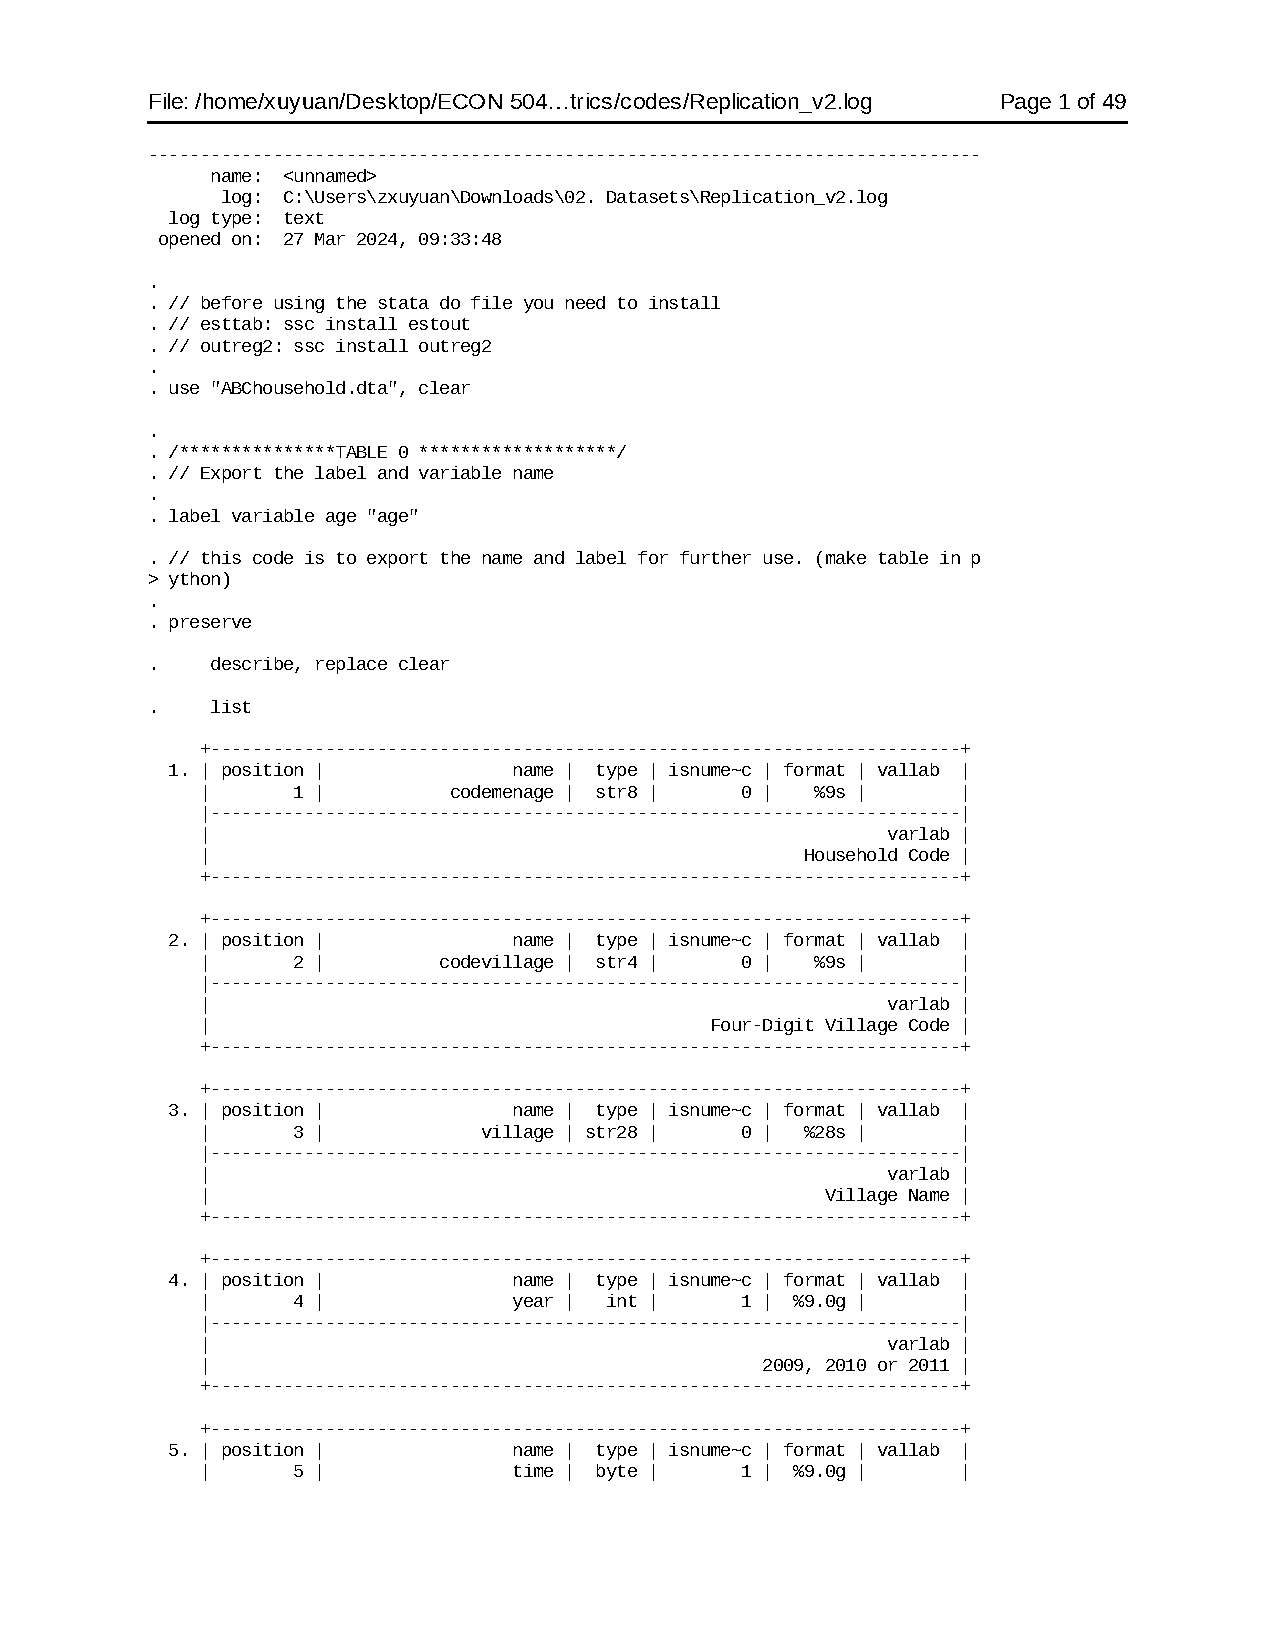
\includepdf[pages=-]{log_file/Replication_v2.log.pdf}
\end{document}
